% This is LLNCS.DEM the demonstration file of
% the LaTeX macro package from Springer-Verlag
% for Lecture Notes in Computer Science,
% version 2.4 for LaTeX2e as of 16. April 2010
%
\documentclass{llncs}
\usepackage{algorithm}
\usepackage{algorithmic}
\usepackage{epsfig}
\usepackage{graphicx}
\usepackage{xcolor}
\usepackage{amsfonts,amsmath,amssymb}
\usepackage{fixltx2e} % Fixing numbering problem when using figure/table* 
\usepackage{booktabs}
\usepackage{tabularx}

%
\usepackage{makeidx}  % allows for indexgeneration
%
\begin{document}
%
\mainmatter              % start of the contributions
%
\title{Time Series Classification Using SAX Representation and Vector Space Model.}
%
\titlerunning{Timeseries features discovery with SAX and TF-IDF weighting}  % abbreviated title (for running head)
%                                     also used for the TOC unless
%                                     \toctitle is used
%
\author{Pavel Senin\inst{1}
\and Sergey Malinchik\inst{2}
}
%
\authorrunning{Pavel Senin} % abbreviated author list (for running head)
%
%%%% list of authors for the TOC (use if author list has to be modified)
%\tocauthor{Ivar Ekeland, Roger Temam, Jeffrey Dean, David Grove,
%Craig Chambers, Kim B. Bruce, and Elisa Bertino}
%
\institute{Collaborative Software Development Laboratory,\\
Information and Computer Sciences Department,\\
University of Hawaii at Manoa,\\ Honolulu HI 96822, USA,\\
\email{senin@hawaii.edu}
\and
Lockheed Martin Advanced Technology Laboratories,\\
Executive Campus, Suite 600, Cherry Hill, NJ 08002, USA,\\
\email{sergey.b.malinchik@lmco.com}}


\maketitle              % typeset the title of the contribution

\begin{abstract}
Ability to discover characteristic patterns in time series paves the road for many downstream
analyses such as classification and clustering, while enabling interpretability of results. 

In this paper, we propose a novel method for time series features discovery based on two existing
techniques - Symbolic Aggregate Approximation (SAX) and Vector space model. 
This method is capable automatically discover and rank time series patterns by their “importance” to
the class, which not only creates well-performing classifiers, but, in turn, provides interpretable
class generalization and facilitates clustering. The accuracy of this technique, as shown  through
our experimental evaluation, is matching current state of the art while being extremely robust to
noise and lost values.  

While being relatively computationally expensive within a learning phase, our method provides fast,
precise, and interpretable classification.
\keywords{Knowledge discovery, Algorithms, Experimentation}
\end{abstract}
%
\section{Introduction}
%
Time series classification is an increasingly popular area of the research. While there are numerous
algorithms proposed within recent years, to date, the most robust method is the simple nearest
neighbor algorithm (KNN) built upon Euclidean distance or DTW \cite{1NN}, which is simple, and
depends on a very few parameters \cite{ed}.
However, while being virtually unbeatable in performance, kNN algorithm requires significant time
and space resources. Another drawback is that it provides a very little information about why the
particular time-series was assigned to a particular class except to their mutual distance metrics.
Also, it was shown, that it is possible to perform better in classification and clustering with more
adaptive distance metrics.

As an alternative to kNN algorithm, recently, time series shapelets were introduced \cite{shapelet}.
A shapelet is a short time series subsequence that is a representative of class membership - a class
characteristic feature. Instead of iteratively looking for the closest neighbor among all known
instances, shapelets-based approaches classifies unknown sequences by use of a multivariate
decision-tree, that supports branching based on conjunctions or disjunctions of shapelets
\cite{logical}. 
While demonstrating a superior interpretability, robustness, and being similar to kNN algorithm
in performance, shapelets-based approaches are outperformed by other classifiers
and require some additional tuning. Moreover, the approach is somewhat time-consuming,  since it
requires an extensive search for best shapelet(s) in order to build a classification tree.

In this work, we propose a similar to shapelets technique, which is also rests on finding time
series subsequences that are representatives of classes. However, instead of recursive search for a
set of shapelets, our technique finds and weights by importance all possible subsequences at once.

\section{Background}
Our methodology is based on two well-known techniques. The first technique is Symbolic Aggregate
approXimation \cite{sax}, which is a high-level, low-bounding symbolic representation of time series
data. The second technique is a Vector Space model and TF*IDF statistics \cite{salton}.

\subsection{Symbolic Aggregate approXimation (SAX)}
Symbolic representation of time series, once introduced \cite{sax}, has attracted much attention,
because it opened the door for application of numerous string-processing algorithms, bioinformatics
and text data mining tools. In addition, this method provides significant reduction of the
dimensionality and is low-bounding to Euclidean distance as shown by Lin \& Keogh, which guarantees
no false-dismissal.

SAX is based on the assumption that normalized time series tend to have have Gaussian distribution
\cite{larsen_marx}, so by determining the breakpoints that correspond to the chosen alphabet
size, one can obtain equal sized areas under the Gaussian curve. Algorithm consists of following
steps: in the first step the time series (or a sub-series) is normalized. In the second step, the
dimensionality of the time series is reduced by using the PAA \cite{paa}. In PAA, times series is
divided into equally sized segments, and the mean values of the points within segments then computed
and constitute a lower dimensional vector - which represents the original time series. Finally, in
the third step, the PAA representation of the time series is discretized into the string by use of
lookup tables and the PAA values.

Note, that in further SAX development \cite{hot_sax}for application to problem of discords
and motifs discovery, streams analyses and clustering \cite{streaming_sax}, authors
proposed a sampling strategy and a distance function specifically designed in order to avoid trivial
and degenerative solutions. 

\subsection{Bag of words, documents corpus}
“Bag of words” is a widely used term in IR. Although, similar definitions, such as “bag of features”
\cite{bag_features} or “bag of patterns” \cite{bag_patterns} were previously proposed for techniques
built upon SAX, we  will use “bag of words” since it reflects symbolic space. Essentially, in our
algorithm                                                                                      and
in our implementation bag of words is a hashmap which maps extracted y SAX words (a
“term”) to their observed frequencies. Set of such bags, representing all TRAIN classes, orms a
“corpus” which is used in downstream steps.

Note, that just as in Linguistics, such a corpus could be built from bags of SAX words obtained with
different parameters, or, moreover, by parsing every single series by more than once. This,
potentially, not only improves performance of our technique, but also facilitates multivariate
series classification.

\subsection{Vector Space Model (VSM)}
We use the vector space model exactly as it is known in information retrieval, for
disambiguating class entities \cite{salton}. Bags of words, representing each of the training
classes, are converted into the vectors whose dimensions correspond to separate “terms” - observed
in a corpus SAX words. 

We employ the \textit{tf$\ast$idf} weighting scheme for terms (SAX words) ranking 
which is defined for a term $t$ and document $D$ 
as a product of a logarithm of a raw term frequency in a document $D$:
\begin{equation}
 \mbox{w}_{t, D} =  \begin{cases} 1 + \log(\mbox{tf}_{t,D}), & \mbox{if } tf_{t,D}>0  \\ 0, & \mbox{otherwise } \end{cases}
\end{equation} 
and a logarithm of an inverse document frequency for that term:
\begin{equation}
 idf_{t} =  \log_{10}(\frac{N}{\mbox{df}_{t}})
\end{equation} 

\section{Our algorithm, SAX-VSM}
Our classification algorithm consists of two distinct phases - the training phase and the
classification itself. The training phase is relatively computationally expensive because it
involves extraction of SAX words from all known series and their post-processing with VSM.
However, there is no need to maintain an index of training series or to store them in memory -
algorithm simply iterates over all labeled series, one by one, building bags of SAX words.
Once built, the corpus is processed with \textit{tf$\ast$idf}, which results in $N$
real-valued vectors needed for for classification (where $N$ is the number of classes).

The classification procedure itself is fast and consists of converting each of the unknown series
into a vector of terms frequencies, which, in turn, is classified by computing $N$ cosine values
(where $N$ is the number of classes) and assigning a series to the class with which cosine is
maximal (i.e angle is minimal).

\subsection{Training phase}
In order to employ Information Retrieval techniques, we transform all training instances from a
single TRAIN class into the single bag of words. For this, our algorithm converts a real valued time
series into SAX string representation configured by five parameters: the sliding window length (w),
the number of PAA frames per window (p), the SAX alphabet size (a), and by the complexity reduction
strategy (s). Note, that each subseries, extracted with sliding window is normalized by energy
before being processed with PAA \cite{goldin_kanellakis}. If, however, the standard deviation is
below a fixed epsilon, similarly to SAX approach, we do not apply normalization
\cite{sax}. Further we shall discuss the parameters selection procedure in the following section.

By applying this procedure to all N training classes, we build a corpus of N bags (or documents in
IR terms), which in turn we process with \textit{tf$\ast$idf}. This provides N vectors, each of
which is a characteristic representative of a class. \textit{tf$\ast$idf} statistics naturally
``highlights’’ class terms bearing unique to the class features (in our context - curves) by
assigning higher weight. Contrary, it ``cancels’’ those terms, which present in the majority of
classes by assigning low weights. Note however, that this weights are not binary (need to refer to
shapelets?), the range of their values is continuous, facilitating smooth boundaries between
classes, which allows to define outliers (i.e. series which are not representatives of any of known
classes).

Intuitively, \textit{tf$\ast$idf} statistic ``refines’’ frequency-based vector space model by
elevating weight coefficients for terms which are true representative of the class, while lowering
weights for terms tend to ``confuse’’ a classier.

Once N vectors are weighted with \textit{tf$\ast$idf}, they are normalized and used in the
classification procedure.

\subsection{Classification}
Similarly to training phase, in order to classify an unknown time-series, we transform it into the
terms vector using the same SAX parameters which we have used in training phase. Then, we compute
cosine values between this vector and those built in the training phase - which represent $N$ known
classes. The series is then assigned to the class whose vector yields the maximal cosine similarity
value.

\section{Results}
We have proposed a novel algorithm for time series classification based on the SAX
representation of time series and Vector space model called SAX-VSM. Here we present a range of
experiments assessing its performance for classification and clustering.

\section{Classification}
To evaluate our approach, we selected XX data sets from the UCR time series repository.
We selected these particular data sets with intention to evaluate the performance of our approach
not only against 1NN Euclidean and DTW classifiers, but recently proposed shapelet decision trees
and a shapelet transform \cite{bagnal}.
We used train/test split and all reported results are testing accuracy. All SAX parsing parameters
and the bag construction strategy were found exclusively on a training set in leave one out 
cross-validation fashion. The test set was used only once with the final set of parameters. 
Our algorithm implementation is publicly available at \cite{jmotif}.

{\scriptsize

\begin{tabular}{|  l | c | c | c | c | c |  c | }
  \hline
  Dataset & 1NN-Eu & 1NN-DTW & 1NN-SAX & Shapelet Tree & Shapelet SVM & SAX-VSM \\
  \hline
  SyntheticControl  & 0.12  & \textbf{0.007} & 0.02 & 5.77 & 12.77 & 0.013 \\
  
\end{tabular}

}

\subsection{}
\begin{figure}[tbp]
   \centering
   \includegraphics[width=130mm]{figures/precision-runtime.ps}
   \caption{Precision-Runtime}
   \label{fig:precision-runtime}
\end{figure}

\subsection{Exploratory analysis of classifier}
We use a well-studied \textit{Gun Point} dataset to show the interpretability of real-life
classification results. The \textit{Gun Point} data contains time series of an actor performing the
motion of drawing a gun, and the classification problem is to determine whether or not she were
holding a gun or imitated the action (the \textit{Gun/NoGun problem}). In \cite{shapelet}, they
identified that the best shapelet for classification was when the actor lowered her arm without a
gun - the ``overshoot'' phenomena causing the dip in the time series. In \cite{bagnal}, when
reporting 10 best shapelets for a similar problem, they confirmed the phenomena with 7 shapelets,
adding 3 shapelets reflecting arm rising motion with a gun. Both shapelets clusters are confirmed by
our approach as shown at the Figure \ref{fig:shapelet-like-patterns}, moreover, in the \textit{Gun}
set, our approach also highlighted the upward arm motion.

\begin{figure}[tbp]
   \centering
   \includegraphics[width=130mm]{figures/shapelet-patterns.ps}
   \caption{The two best weighted sub-series from each class of Gun Point dataset. 
   Note, the upward arm motion is more ``important'' in a Gun set, whether downward arm motion in
NoGun set. These result aligns with previous work \cite{bagnal} reporting best shapelets at this
locations.
}
   \label{fig:shapelet-like-patterns}
\end{figure}

\section{Conclusion}
In our opinion, the superior classification performance of our approach is based on 
a number of factors. 
First of all, our approach is very different in nature from those 
based on convenient distance measures such as Euclidean distance or DTW - to some 
extent we do not pay attention to ordering of time points outside of sliding window. 
Surely, overlapping windows do carry information about initial ordering, but this 
is fading away along the steps of our algorithm.
Secondly, we are able to efficiently tolerate noise by leveraging agglomeration 
and mediation with PAA. 
Thirdly, the SAX alphabet cuts provide flexible boundaries for capturing similar 
sub-series. 
And finally, Vector space model and textit{tf$\ast$idf} statistics provide us 
with efficient discrimination and measurement toolkit: the tf part of the weighting scheme
captures the frequency of observed feqtures within the class, while the idf part 
captures the feature informativeness (features that appear in many classes 
are less informative than those that appear rarely)

\begin{algorithm}
\caption{Class Bag of Words construction}
\label{alg1}
\begin{algorithmic}[1]
\REQUIRE A dataset $D$ containing at least one time series
\ENSURE Return a class WordBag
\STATE $W \leftarrow$ sliding window size
\STATE $P \leftarrow$ PAA size
\STATE $A \leftarrow$ SAX alphabet size
\STATE $B \leftarrow$ \{the resulting bag\}
\FOR{ $t$ in $D$}
 \FOR{ $i\leftarrow 1$ to $|t|-W$}
 \STATE $w \leftarrow SAX(subseries(t,i,W), P, A))$ \{convert subseries into word\}
 \STATE $B \leftarrow w$ \{put the word into the bag, updating frequency\}
 \ENDFOR
\ENDFOR
\RETURN $B$
\end{algorithmic}
\end{algorithm}

%
% ---- Bibliography ----
%
\begin{thebibliography}{5}
%

\bibitem {ed}
Ding, H., Trajcevski, G., Scheuermann, P., Wang, X., Keogh, E.:
Querying and mining of time series data: experimental comparison of representations and distance measures,
Proc. VLDB Endow., 1542--1552 (2008)

\bibitem {1NN}
Xi, X., Keogh, E., Shelton, C., Wei, L., Ratanamahatana, C.A.:
Fast time series classification using numerosity reduction,
Proceedings of the 23rd international conference on Machine learning (ICML '06). 
NY, USA, 1033-1040.

\bibitem {shapelet}
Ye, L., Keogh, E.:
Time series shapelets: a new primitive for data mining.
Proceedings of the 15th ACM SIGKDD international conference on Knowledge discovery and data mining,
Paris, France, 947--956, (2009)

\bibitem {logical}
Mueen, A., Keogh, E., Young, N.:
Logical-shapelets: an expressive primitive for time series classification.
Proceedings of the 17th ACM SIGKDD international conference on Knowledge discovery and data mining,
San Diego, California, USA, 1154--1162, (2011)

\bibitem {sax}
Lin, J., Keogh, E., Wei, L., Lonardi, S.:
Experiencing SAX: a novel symbolic representation of time series.
Data Mining and Knowledge Discovery, 107--144, (2007)

\bibitem {salton}
Salton, G., Wong, A., Yang., C.S.,:
A vector space model for automatic indexing. 
Commun. ACM 18, 11, 613--620, (November 1975)

\bibitem {larsen_marx}
Larsen, Richard J. and Marx, Morris L.:
An Introduction to Mathematical Statistics and Its Applications (3rd Edition)
Prentice Hall, 2000.

\bibitem {paa}
Keogh, E., Pazzani, M.J.:
A Simple Dimensionality Reduction Technique for Fast Similarity Search in Large Time Series Databases. 
Proceedings of the 4th Pacific-Asia Conference on Knowledge Discovery and Data Mining, Current Issues and New Applications (PADKK '00), 
Takao Terano, Huan Liu, and Arbee L. P. Chen (Eds.). Springer-Verlag, London, UK, UK, 122-133.

\bibitem {hot_sax}
Keogh, E., Lin, J., Fu, A.:
HOT SAX: Efficiently Finding the Most Unusual Time Series Subsequence. 
Proceedings of the Fifth IEEE International Conference on Data Mining (ICDM'05). 
IEEE Computer Society, Washington, DC, USA, 226-233.

\bibitem {streaming_sax}
Lin, J., Keogh, E., Lonardi, S., Chiu, B.:
A symbolic representation of time series, with implications for streaming algorithms. 
Proceedings of the 8th ACM SIGMOD workshop on Research issues in data mining and knowledge discovery (DMKD '03).
ACM, New York, NY, USA, 2-11.

\bibitem {bag_features}
Lin, J., Khade, R., Li, Y.:
Finding Structural Similarity in Time Series Data Using Bag-of-Patterns Representation. 
Proceedings of the 21st International Conference on Scientific and Statistical Database Management (SSDBM 2009),
Marianne Winslett (Ed.). Springer-Verlag, Berlin, Heidelberg, 461-477.

\bibitem {bag_patterns}
Lin, J., Khade, R., Li, Y.:
Rotation-invariant similarity in time series using bag-of-patterns representation. 
J. Intell. Inf. Syst. 39, 2 (October 2012), 287-315.

\bibitem {goldin_kanellakis}
D.Q., Kanellakis, P.C.,:
On Similarity Queries for Time-Series Data: Constraint Specification and Implementation. 
Proceedings of the First International Conference on Principles and Practice of Constraint Programming (CP '95), 
Ugo Montanari and Francesca Rossi (Eds.). Springer-Verlag, London, UK, UK, 137-153.

\bibitem {bagnal}
Lines, J., Davis, L.M., Hills, J., Bagnall, A.:
A shapelet transform for time series classification. 
In Proceedings of the 18th ACM SIGKDD international conference on Knowledge discovery and data mining (KDD '12). 
ACM, New York, NY, USA, 289-297.


\bibitem {jmotif}
paper Authors: 
Accompanying information for this paper. 
https://code.google.com/p/jmotif/

\end{thebibliography}

%\clearpage
%\addtocmark[2]{Author Index} % additional numbered TOC entry
%\renewcommand{\indexname}{Author Index}
%\printindex
%\clearpage
%\addtocmark[2]{Subject Index} % additional numbered TOC entry
%\markboth{Subject Index}{Subject Index}
%\renewcommand{\indexname}{Subject Index}
%\input{subjidx.ind}
\end{document}
